\apendice{Plan de Proyecto Software}

\section{Introducción}

\section{Planificación temporal}
La planificación temporal del proyecto se ha seguido con la realización de los \textit{sprints} marcados en cada reunión.

\subsubsection{\textit{Sprint} 1: \textit{Sprint} inicial}
Fechas: 28 febrero 2023 - 7 marzo 2023
\begin{itemize}
\item\textbf{Planificación del \textit{sprint}}

En la reunión de planificación del sprint se fijaron las siguientes tareas:
\begin{enumerate}
	\item Configuración inicial del repositorio
	\item Prototipos de las vistas de la aplicación
	\item Creación diagrama entidad-relación
\end{enumerate}

\item\textbf{\textit{Burndown Report}}

\begin{figure}[h]
	\centering
	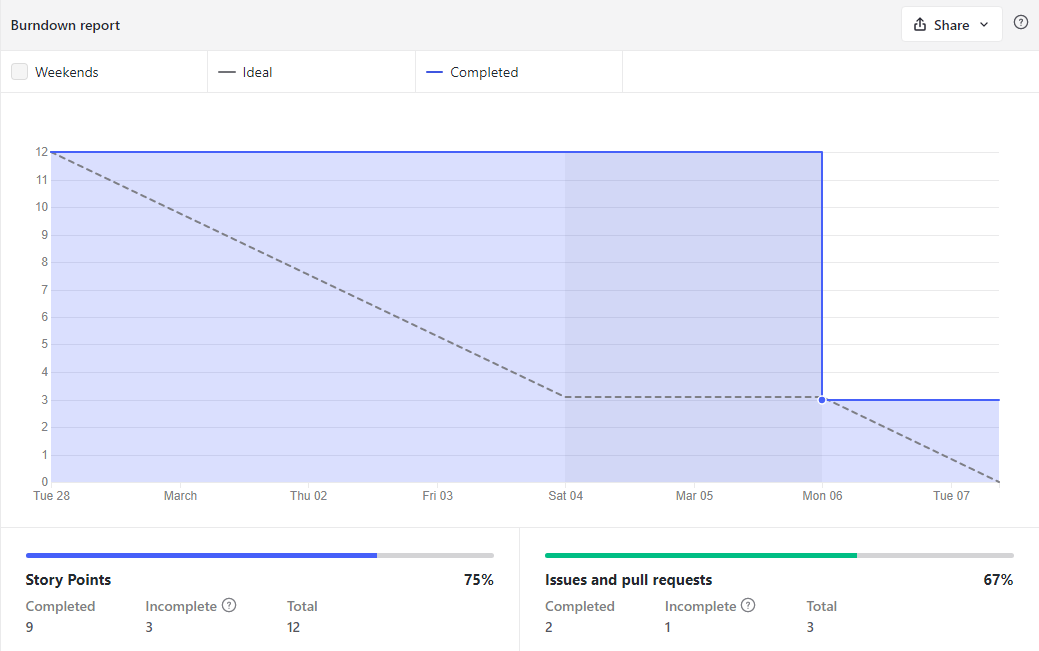
\includegraphics[width=\textwidth]{../img/Anexos/Sprints/Sprint1.png}
	\caption{\textit{Burndown Report Sprint 1}}
\end{figure}
\FloatBarrier
Como se puede apreciar en el gráfico, no todas las tareas aparecen como completadas. Esto es debido a que el diagrama entidad-relación se dejó abierto ya que faltaba información para completarlo y después se fijaron diversos cambios.

\item\textbf{Revisión del \textit{sprint}}

Durante la revisión se mostró el trabajo realizado y se vieron los cambios que se debían realizar en el diagrama entidad-relación que a su vez implicaban cambios en los prototipos de las vistas de la aplicación.
Se llegó a la conclusión de que podía ser buena idea dividir el diagrama E/R haciendo vistas del mismo para que fuere más fácil resolverlo.
\end{itemize}


\subsubsection{\textit{Sprint} 2: Casos de uso y diagrama E/R de cada caso}
Fechas: 7 marzo 2023 - 14 marzo 2023
\begin{itemize}
\item\textbf{Planificación del \textit{sprint}}

En la reunión de planificación del sprint se fijaron las siguientes tareas:
\begin{enumerate}
	\item Creación de casos de uso junto a su vista del diagrama E/R
	\item Aprendizaje de \textit{Flask}
\end{enumerate}

\item\textbf{\textit{Burndown Report}}

\begin{figure}[h]
	\centering
	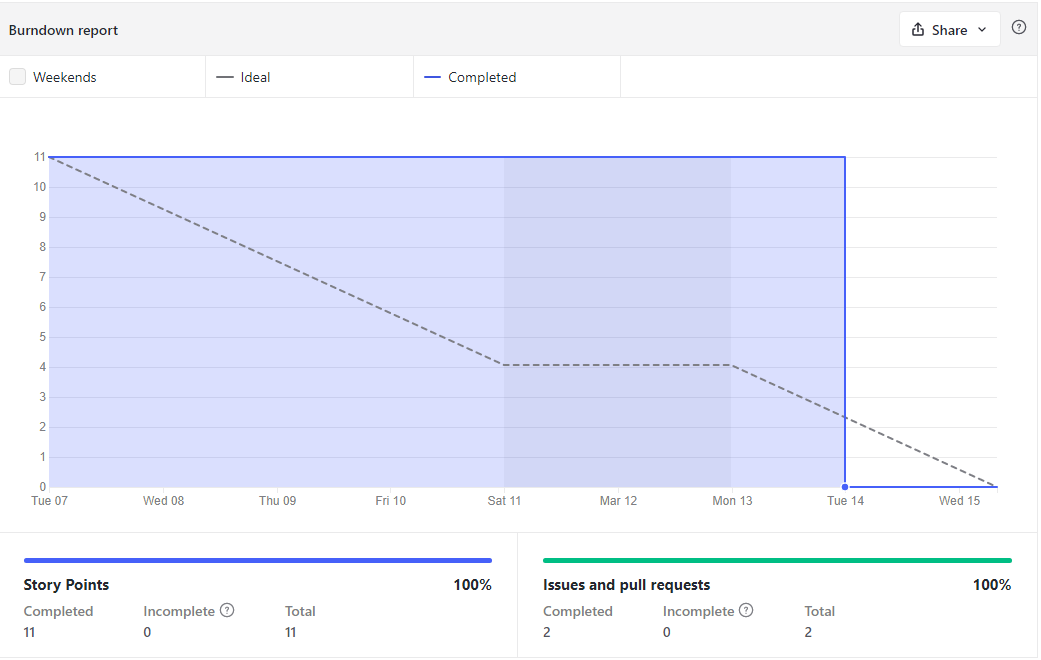
\includegraphics[width=\textwidth]{../img/Anexos/Sprints/Sprint2.png}
	\caption{\textit{Burndown Report Sprint 2}}
\end{figure}
\FloatBarrier
En este \textit{sprint} se completaron las tareas marcadas en el tiempo fijado durante la reunión de planificación, pero muchas cosas quedaron pendientes de cambios en futuros \textit{sprints}.

\item\textbf{Revisión del \textit{sprint}}

En la reunión de revisión se estudió de nuevo el diagrama E/R y se indicaron nuevos cambios menores en el mismo. También se propuso el comenzar a realizar el diagrama de casos de uso y continuar con el estudio de \textit{Flask}.
\end{itemize}

\subsubsection{\textit{Sprint} 3: Documentación de casos de uso e investigación y aprendizaje de \textit{Flask} y bibliotecas \textit{JavaScript}}
Fechas: 14 marzo 2023 - 21 marzo 2023
\begin{itemize}
\item\textbf{Planificación del \textit{sprint}}

En la reunión de planificación del sprint se fijaron las siguientes tareas:
\begin{enumerate}
		\item Realizar el diagrama de casos de uso
		\item Cambios en las vistas adaptándolas a los casos de uso
		\item Documentar los casos de uso con sus tablas
		\item Investigar bibliotecas de JavaScript que pudiesen ayudar
		\item Aprender sobre \textit{Flask}
\end{enumerate}

\item\textbf{\textit{Burndown Report}}

\begin{figure}[h]
	\centering
	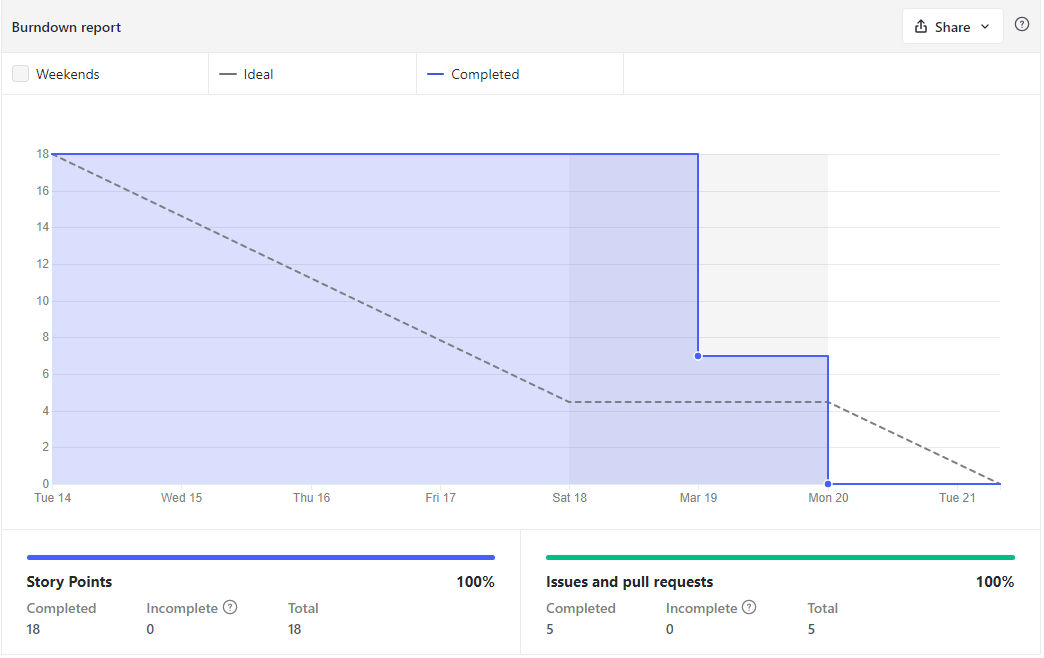
\includegraphics[width=\textwidth]{../img/Anexos/Sprints/Sprint3.png}
	\caption{\textit{Burndown Report Sprint 3}}
\end{figure}
\FloatBarrier
En este \textit{sprint} se completaron las tareas marcadas aunque el tiempo marcado para el aprendizaje de \textit{Flask} fue menor debido a falta de tiempo durante esta semana. Estaba previsto dedicar en total 18 horas al \textit{sprint}, pero finalmente fueron 15.

\item\textbf{Revisión del \textit{sprint}}

Durante la revisión se vio que había casos de uso que no eran necesarios y que se podían añadir como excepciones de otros. Esto produjo que el diagrama de casos de uso se debía cambiar, lo que implica un cambio en la documentación de las tablas y en los prototipos de las vistas de la aplicación.
\end{itemize}



\section{Estudio de viabilidad}

\subsection{Viabilidad económica}

\subsection{Viabilidad legal}


